% Provenance (never printed): cycle 4 SVT, "La planete Terre, l'environnement
% et l'action humaine": the relief as a balance between uplift and erosion;
% landforms of the wind, the sea and dissolution; reading a landscape; see
% sources/book1/PROVENANCE.md. Book 1, grade 9, chapter 4.
% Vocabulary guard: owns uplift, dune, cliff, beach and spit (with longshore
% drift), karst (with cave and sinkhole). Landscape and landform are g1's;
% weathering, erosion, deposition, meander and delta are g5's; relief is
% g4's; plates and mountain building are g7's; U-shaped valley and moraine
% are g8's; limestone and the acid test are g6's; acids are the chemistry
% books' (recalled in prose). Contour lines are g9.5's (not used here).
% "Normal fault" and the destruction of mountains are Book 2's.
\chapter{Les formes du relief}\label{ch:g9:landforms}

Sur la \omterm{def:g1:landscapes-around-us:water}{côte} sud de l'Angleterre, les \omterm{def:g9:landforms:cliff}{falaises} blanches des Seven Sisters
tombent à pic dans la \omterm{def:g2:water-on-earth:ocean}{mer}. Une année normale, elles perdent jusqu'à un
mètre. Pendant l'hiver 2014, les \omterm{def:g5:natural-hazards:storm}{tempêtes} ont arraché aux \omterm{def:g9:landforms:cliff}{falaises} de
Birling Gap, en deux mois, autant qu'elles en perdent d'habitude en sept
ans. La craie de ces \omterm{def:g9:landforms:cliff}{falaises} était autrefois une \omterm{def:g3:stones-pebbles-sand:sand}{boue} au fond d'une \omterm{def:g2:water-on-earth:ocean}{mer},
faite des minuscules \omterm{def:g7:plate-tectonics:plate}{plaques} d'algues microscopiques qui vivaient dans ses
eaux. Elle se dresse aujourd'hui comme un mur de \omterm{def:g3:stones-pebbles-sand:rock}{roche} blanche que les
vagues font reculer un peu plus chaque année. Pourquoi le \omterm{def:g4:world-physical-map:relief}{relief} a-t-il
les formes qu'il a, et pourquoi certaines changent-elles si vite~?
% ledger: nt:birling-2014, sdnp:birling, nasa:coccoliths

\begin{omfigure}
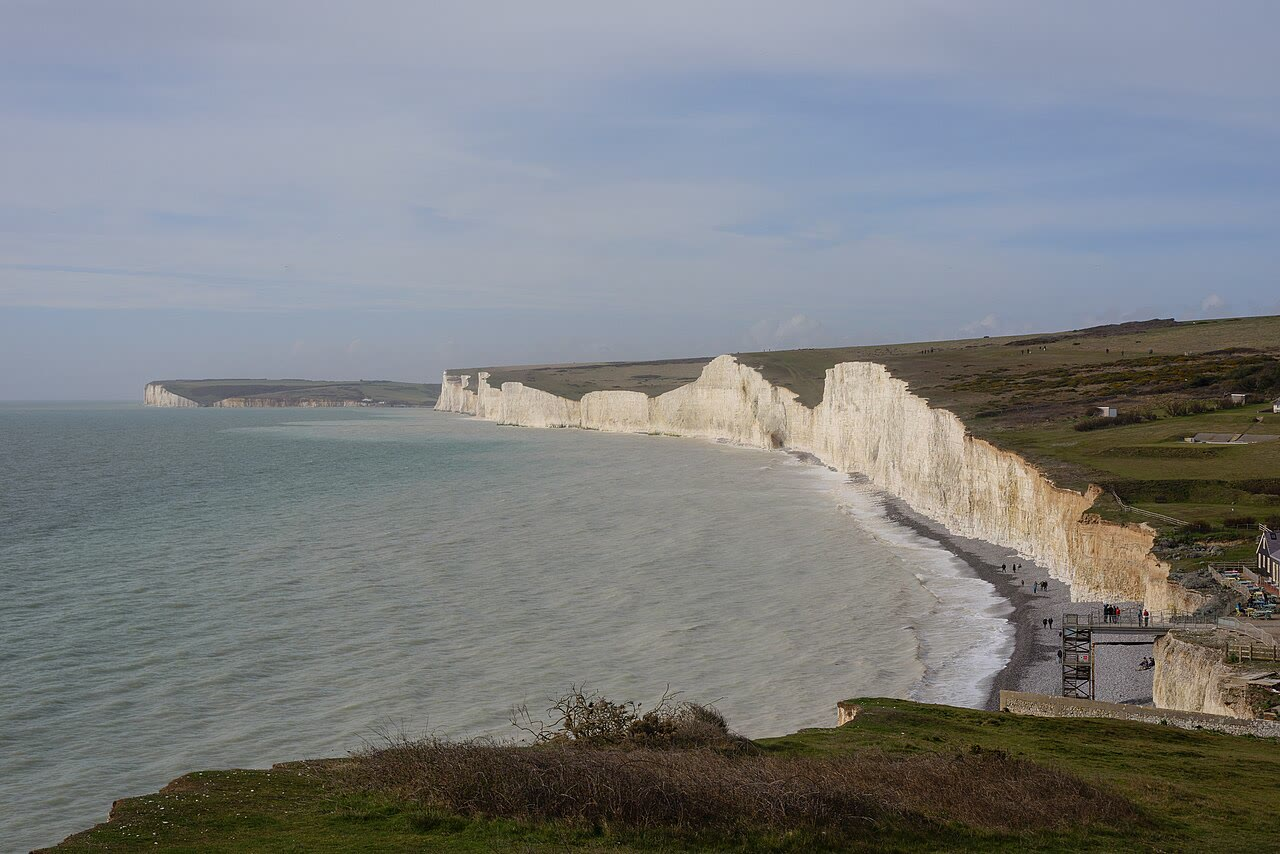
\includegraphics[width=\linewidth]{images/book1/g9-seven-sisters.jpg}

{\small Les Seven Sisters, \omterm{def:g9:landforms:cliff}{falaises} de craie de la \omterm{def:g1:landscapes-around-us:water}{côte} de l'East Sussex
(Angleterre), avec au premier plan les maisons de Birling Gap. Les \omterm{def:g9:landforms:cliff}{falaises}
reculent sous l'action de la \omterm{def:g2:water-on-earth:ocean}{mer}, et des éboulements peuvent se produire
à tout moment. À leur pied s'étend une \omterm{def:g9:landforms:beach}{plage} de \omterm{def:g3:stones-pebbles-sand:pebble}{galets}. Photographie Arild
Vågen, 2017 (CC BY-SA 4.0, via Wikimedia Commons).}
% ledger: commons:seven-sisters, sdnp:birling
\label{fig:g9:landforms:seven-sisters}
\end{omfigure}

\begin{recall}
Une \emph{\omterm{def:g1:landscapes-around-us:landform}{forme de relief}} est l'une des formes du terrain~: une \omterm{def:g1:landscapes-around-us:landform}{colline},
une \omterm{def:g1:landscapes-around-us:landform}{vallée}, une \omterm{def:g1:landscapes-around-us:landform}{plaine}, une \omterm{def:g9:landforms:cliff}{falaise} (\cref{ch:g1:landscapes-around-us}). Le
\omterm{def:g4:world-physical-map:relief}{relief} est la forme du terrain en \omterm{def:g4:world-physical-map:altitude}{altitude} (\cref{ch:g4:world-physical-map}).
L'\omterm{def:g5:water-shapes-the-land:weathering}{altération} fragmente la \omterm{def:g3:stones-pebbles-sand:rock}{roche}, l'\omterm{def:g5:water-shapes-the-land:erosion}{érosion} l'use et l'emporte, et le \omterm{def:g5:water-shapes-the-land:deposition}{dépôt}
la dépose ailleurs (\cref{ch:g5:water-shapes-the-land}). Les \omterm{def:g7:plate-tectonics:plate}{plaques}
soulèvent des \omterm{def:g4:world-physical-map:range}{chaînes de montagnes} là où elles entrent en collision
(\cref{ch:g7:plate-tectonics})~; les \omterm{def:g8:ice-on-earth:glacier}{glaciers} creusent des \omterm{def:g8:ice-on-earth:glacial-landforms}{vallées en U}
(\cref{ch:g8:ice-on-earth})~; le calcaire fait effervescence sous une goutte
d'acide dilué (\cref{ch:g6:rocks-and-minerals}). En chimie, on apprend que
les acides attaquent le calcaire en libérant du dioxyde de carbone.
\end{recall}

\section{Le relief~: un équilibre entre soulèvement et érosion}

Deux sortes de forces façonnent le \omterm{def:g4:world-physical-map:relief}{relief}. De l'intérieur, les mouvements
des \omterm{def:g7:plate-tectonics:plate}{plaques} soulèvent le sol. De l'extérieur, l'eau, la glace, le vent et
la \omterm{def:g2:water-on-earth:ocean}{mer} l'usent.

\begin{definition}[Soulèvement]\label{def:g9:landforms:uplift}
Le \emph{soulèvement}\index{soulevement@soulèvement} est la lente élévation des \omterm{def:g3:stones-pebbles-sand:rock}{roches} et de la
surface du sol d'une région, sous l'effet de forces internes à la Terre,
comme la collision de deux \omterm{def:g7:plate-tectonics:plate}{plaques}.
\end{definition}

Le \omterm{def:g9:landforms:uplift}{soulèvement} est lent à l'échelle d'une vie, mais rapide à l'échelle de
la Terre. L'Inde est entrée en collision avec l'Asie il y a environ
50~millions d'années, et le plateau du Tibet, derrière l'Himalaya, a gagné
l'essentiel de son \omterm{def:g4:world-physical-map:altitude}{altitude}, environ \qty{4600}{m}, au cours des
10~derniers millions d'années. En moyenne, cela fait
$4600 \div 10^7 = 4.6 \times 10^{-4}$~m, soit environ \qty{0.5}{mm} par
an~: moins que l'épaisseur d'un ongle, mais maintenu pendant des millions
d'années.
% ledger: usgs:himalaya (rate computed in figdata/grade-9/cliff_retreat.py, tibet_rate_mm_yr)

Dès que le sol s'élève, l'\omterm{def:g5:water-shapes-the-land:erosion}{érosion} l'attaque. Plus le terrain est haut et
raide, plus les \omterm{def:g1:landscapes-around-us:water}{rivières}, les \omterm{def:g8:ice-on-earth:glacier}{glaciers} et les éboulements emportent vite
la \omterm{def:g3:stones-pebbles-sand:rock}{roche}. L'\omterm{def:g4:world-physical-map:altitude}{altitude} d'une \omterm{def:g4:world-physical-map:range}{chaîne de montagnes} à un moment donné est le
résultat d'une lutte~: ce que le \omterm{def:g9:landforms:uplift}{soulèvement} apporte, moins ce que
l'\omterm{def:g5:water-shapes-the-land:erosion}{érosion} enlève.

\begin{omfigure}
\begin{tikzpicture}[font=\footnotesize, >={Stealth[length=2mm]}]
  % panel 1: uplift faster than erosion
  \begin{scope}
    \fill[black!13] (0,0) -- (0.5,0) .. controls (1.1,1.0) and (1.5,2.0) .. (1.8,2.2)
      .. controls (2.1,2.0) and (2.5,1.0) .. (3.1,0) -- (3.6,0) -- (3.6,-0.5) -- (0,-0.5) -- cycle;
    \draw[black!60] (0,0) -- (0.5,0) .. controls (1.1,1.0) and (1.5,2.0) .. (1.8,2.2)
      .. controls (2.1,2.0) and (2.5,1.0) .. (3.1,0) -- (3.6,0);
    \draw[black!60, dashed] (0.7,0) .. controls (1.2,0.8) and (1.5,1.5) .. (1.8,1.6)
      .. controls (2.1,1.5) and (2.4,0.8) .. (2.9,0);
    \foreach \x in {1.2,1.8,2.4} \draw[->, omWarm, line width=1.4pt] (\x,-0.45) -- ++(0,1.0);
    \draw[->, omRiver, thick] (2.15,1.6) -- ++(0.35,-0.3);
    \node[align=center, anchor=north] at (1.8,-0.6) {soulèvement plus\\rapide que l'érosion~:\\le relief s'élève};
  \end{scope}
  % panel 2: uplift equals erosion
  \begin{scope}[xshift=4.4cm]
    \fill[black!13] (0,0) -- (0.5,0) .. controls (1.1,1.0) and (1.5,1.8) .. (1.8,1.9)
      .. controls (2.1,1.8) and (2.5,1.0) .. (3.1,0) -- (3.6,0) -- (3.6,-0.5) -- (0,-0.5) -- cycle;
    \draw[black!60] (0,0) -- (0.5,0) .. controls (1.1,1.0) and (1.5,1.8) .. (1.8,1.9)
      .. controls (2.1,1.8) and (2.5,1.0) .. (3.1,0) -- (3.6,0);
    \foreach \x in {1.2,1.8,2.4} \draw[->, omWarm, line width=1.4pt] (\x,-0.45) -- ++(0,0.6);
    \draw[->, omRiver, thick] (2.05,1.6) -- ++(0.55,-0.5);
    \draw[->, omRiver, thick] (1.55,1.6) -- ++(-0.55,-0.5);
    \node[align=center, anchor=north] at (1.8,-0.6) {soulèvement et érosion\\égaux~: l'altitude\\reste la même};
  \end{scope}
  % panel 3: no more uplift
  \begin{scope}[xshift=8.8cm]
    \fill[black!13] (0,0) -- (0.4,0) .. controls (1.1,0.5) and (1.5,0.95) .. (1.8,1.0)
      .. controls (2.1,0.95) and (2.5,0.5) .. (3.2,0) -- (3.6,0) -- (3.6,-0.5) -- (0,-0.5) -- cycle;
    \draw[black!60] (0,0) -- (0.4,0) .. controls (1.1,0.5) and (1.5,0.95) .. (1.8,1.0)
      .. controls (2.1,0.95) and (2.5,0.5) .. (3.2,0) -- (3.6,0);
    \draw[black!60, dashed] (0.5,0) .. controls (1.1,1.0) and (1.5,1.8) .. (1.8,1.9)
      .. controls (2.1,1.8) and (2.5,1.0) .. (3.1,0);
    \draw[->, omRiver, thick] (2.05,0.95) -- ++(0.55,-0.5);
    \draw[->, omRiver, thick] (1.55,0.95) -- ++(-0.55,-0.5);
    \node[align=center, anchor=north] at (1.8,-0.6) {plus de soulèvement~:\\l'érosion abaisse\\le relief};
  \end{scope}
  % key
  \draw[->, omWarm, line width=1.4pt] (13.2,1.2) -- ++(0,0.6) node[right, black] {soulèvement};
  \draw[->, omRiver, thick] (13.2,0.7) -- ++(0.35,-0.3) node[right, black] {érosion};
  \draw[black!60, dashed] (13.1,-0.1) -- ++(0.5,0) node[right, black] {ancien profil};
\end{tikzpicture}

{\small Le \omterm{def:g4:world-physical-map:relief}{relief} comme un équilibre (un croquis, sans souci d'échelle). Le
\omterm{def:g9:landforms:uplift}{soulèvement} élève les \omterm{def:g3:stones-pebbles-sand:rock}{roches}~; l'\omterm{def:g5:water-shapes-the-land:erosion}{érosion} les emporte vers les \omterm{def:g1:landscapes-around-us:landform}{vallées} et la
\omterm{def:g2:water-on-earth:ocean}{mer}. Une chaîne continue de grandir tant que le \omterm{def:g9:landforms:uplift}{soulèvement} l'emporte~;
quand les \omterm{def:g7:plate-tectonics:plate}{plaques} cessent de pousser, l'\omterm{def:g5:water-shapes-the-land:erosion}{érosion} l'use lentement jusqu'à
n'en laisser que des \omterm{def:g1:landscapes-around-us:landform}{collines}.}
\label{fig:g9:landforms:balance}
\end{omfigure}

Les \omterm{def:g1:landscapes-around-us:water}{rivières} (\cref{ch:g5:water-shapes-the-land}) et les \omterm{def:g8:ice-on-earth:glacier}{glaciers}
(\cref{ch:g8:ice-on-earth}) sont les grands sculpteurs des \omterm{def:g1:landscapes-around-us:landform}{montagnes}. La
suite de ce chapitre suit trois autres agents, qui façonnent leurs propres
\omterm{def:g1:landscapes-around-us:landform}{formes de relief}~: le vent, la \omterm{def:g2:water-on-earth:ocean}{mer}, et l'eau qui dissout la \omterm{def:g3:stones-pebbles-sand:rock}{roche}.

\section{Les formes de relief dues au vent~: les dunes}

Là où les plantes sont rares, le \omterm{def:g3:stones-pebbles-sand:sand}{sable} meuble abondant et le vent fort, le
vent peut soulever le \omterm{def:g3:stones-pebbles-sand:sand}{sable} et l'entasser en \omterm{def:g1:landscapes-around-us:landform}{collines}~: dans les \omterm{def:g5:weather-and-climate:desert}{déserts},
et en arrière des \omterm{def:g9:landforms:beach}{plages} de \omterm{def:g3:stones-pebbles-sand:sand}{sable}.
% ledger: nps:aeolian

\begin{definition}[Dune]\label{def:g9:landforms:dune}
Une \emph{dune}\index{dune} est un monticule ou une crête de \omterm{def:g3:stones-pebbles-sand:sand}{sable} meuble
entassé par le vent. Sa pente tournée vers le vent est longue et douce~;
son autre versant, la \emph{face d'avalanche}\index{face d'avalanche}, est
court et raide.
\end{definition}
% ledger: nps:aeolian, nmt:barchan

Une \omterm{def:g9:landforms:dune}{dune} se déplace. Le vent fait rouler et rebondir les grains le long de
la pente douce~; à la crête, ils s'entassent jusqu'à ce que le tas devienne
trop raide, et une petite avalanche de \omterm{def:g3:stones-pebbles-sand:sand}{sable} glisse sur la \omterm{def:g9:landforms:dune}{face
d'avalanche}. Grain après grain, le \omterm{def:g3:stones-pebbles-sand:sand}{sable} est pris du côté exposé au vent
et déposé de l'autre côté, et toute la \omterm{def:g9:landforms:dune}{dune} avance dans le sens du vent
sans jamais être soulevée. Les \omterm{def:g9:landforms:dune}{dunes} sont rarement isolées~: elles
couvrent des champs entiers.
% ledger: nmt:barchan, nps:aeolian

Là où le vent souffle toujours de la même direction et où le \omterm{def:g3:stones-pebbles-sand:sand}{sable} n'est
pas trop abondant, les \omterm{def:g9:landforms:dune}{dunes} prennent la forme d'un croissant, une
\emph{barkhane}~: son nez arrondi fait face au vent et ses deux cornes
pointent dans le sens du vent. Les cornes contiennent moins de \omterm{def:g3:stones-pebbles-sand:sand}{sable} que
le milieu, si bien qu'elles avancent plus vite et s'étirent en avant de la
\omterm{def:g9:landforms:dune}{dune}.
% ledger: nmt:barchan

\begin{omfigure}
\begin{tikzpicture}[font=\footnotesize, >={Stealth[length=2mm]}]
  % plan view
  \fill[yellow!25!orange!20] (3.4,1.3) .. controls (1.0,1.3) and (0.2,0.6) .. (0.2,0)
     .. controls (0.2,-0.6) and (1.0,-1.3) .. (3.4,-1.3)
     .. controls (2.4,-0.9) and (1.8,-0.5) .. (1.8,0)
     .. controls (1.8,0.5) and (2.4,0.9) .. (3.4,1.3) -- cycle;
  \fill[orange!45] (3.4,1.3) .. controls (2.4,0.9) and (1.8,0.5) .. (1.8,0)
     .. controls (1.8,-0.5) and (2.4,-0.9) .. (3.4,-1.3)
     .. controls (2.1,-0.8) and (1.45,-0.45) .. (1.45,0)
     .. controls (1.45,0.45) and (2.1,0.8) .. (3.4,1.3) -- cycle;
  \draw[black!60] (3.4,1.3) .. controls (1.0,1.3) and (0.2,0.6) .. (0.2,0)
     .. controls (0.2,-0.6) and (1.0,-1.3) .. (3.4,-1.3)
     .. controls (2.4,-0.9) and (1.8,-0.5) .. (1.8,0)
     .. controls (1.8,0.5) and (2.4,0.9) .. (3.4,1.3);
  \draw[black, thick] (3.4,1.3) .. controls (2.1,0.8) and (1.45,0.45) .. (1.45,0)
     .. controls (1.45,-0.45) and (2.1,-0.8) .. (3.4,-1.3);
  \foreach \y in {-0.8,0,0.8} \draw[->, omRiver, thick] (-1.3,\y) -- ++(1.1,0);
  \node[above] at (-0.75,0.85) {vent};
  \node[anchor=west] at (3.5,1.35) {corne};
  \node[anchor=west] at (3.5,-1.35) {corne};
  \draw[black!70] (1.75,0.25) -- (2.9,0.35) node[anchor=west, align=left, black] {face d'avalanche\\(raide)};
  \draw[black!70] (0.75,-0.2) -- (0.6,-1.6) node[anchor=north, align=center, black] {pente au vent\\(douce)};
  \draw[black!70] (1.47,-0.3) -- (2.4,-1.75) node[anchor=north, black] {crête};
  \node[anchor=south, font=\footnotesize\bfseries] at (1.4,1.6) {vue de dessus};
  % profile
  \begin{scope}[xshift=7.2cm, yshift=-0.8cm]
    \draw[black!60] (-0.4,0) -- (5.6,0);
    \fill[yellow!25!orange!20] (0,0) -- (3.0,1.2) -- (3.6,0) -- cycle;
    \draw[black!70] (0,0) -- (3.0,1.2) -- (3.6,0);
    \fill[orange!45] (3.0,1.2) -- (3.6,0) -- (3.3,0) -- cycle;
    \draw[black!50, dashed] (0.8,0) -- (3.8,1.2) -- (4.4,0);
    \draw[->, black!70] (0.5,0.35) .. controls (0.75,0.65) .. (1.0,0.45);
    \draw[->, black!70] (1.0,0.55) .. controls (1.25,0.85) .. (1.5,0.65);
    \draw[->, black!70] (1.5,0.75) .. controls (1.75,1.05) .. (2.0,0.85);
    \draw[->, black!70] (2.0,0.95) .. controls (2.25,1.25) .. (2.5,1.05);
    \draw[->, thick, black!80] (3.15,1.05) -- (3.45,0.35);
    \foreach \y in {1.6,2.1} \draw[->, omRiver, thick] (-0.8,\y) -- ++(1.1,0);
    \node[above] at (-0.25,2.1) {vent};
    \draw[->, thick] (4.5,0.6) -- ++(0.7,0) node[right, align=left] {la dune\\avance};
    \node[align=center, anchor=north] at (1.2,-0.1) {les grains\\rebondissent sur\\la pente douce};
    \node[align=center, anchor=north west] at (2.9,-0.1) {puis glissent\\sur la face\\d'avalanche};
    \node[anchor=south, font=\footnotesize\bfseries] at (2.2,2.3) {vue de profil};
  \end{scope}
\end{tikzpicture}

{\small Une \omterm{def:g9:landforms:dune}{dune} en croissant, ou barkhane (un croquis). Vues de dessus, ses
cornes pointent dans le sens du vent. Vus de profil, les grains remontent
la pente douce exposée au vent et glissent sur la \omterm{def:g9:landforms:dune}{face d'avalanche}, raide~:
la \omterm{def:g9:landforms:dune}{dune} avance dans le sens du vent (contour en tirets~: la \omterm{def:g9:landforms:dune}{dune} un peu
plus tard).}
% ledger: nmt:barchan, nps:aeolian
\label{fig:g9:landforms:barchan}
\end{omfigure}

À quelle vitesse~? Dans le champ de \omterm{def:g9:landforms:dune}{dunes} de gypse de White Sands, au
Nouveau-Mexique, les petites \omterm{def:g9:landforms:dune}{dunes} qui se forment à son bord exposé au
vent, hautes de quelques mètres, avancent jusqu'à \qty{6}{m} par an~; un
peu plus loin, devenues hautes de 6 à \qty{10}{m}, elles avancent
d'environ \qty{3}{m} par an. Plus une \omterm{def:g9:landforms:dune}{dune} contient de \omterm{def:g3:stones-pebbles-sand:sand}{sable}, plus elle
est lente. Des barkhanes poussées par des vents forts peuvent parcourir
plus de \qty{100}{m} en un an, assez pour ensevelir une route ou un champ.
% ledger: nps:whsa-migration, nmt:barchan

\begin{omfigure}
\begin{minipage}[c]{0.5\linewidth}\centering
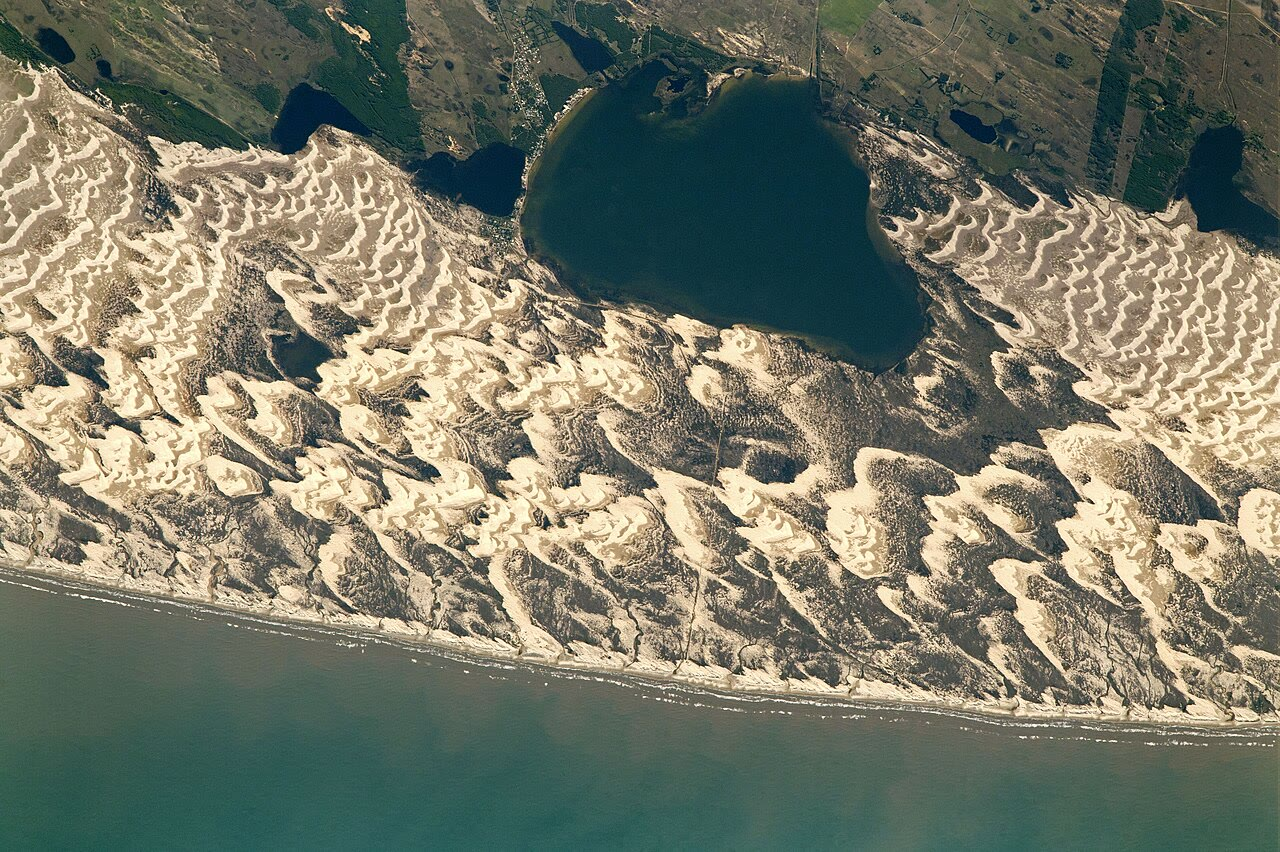
\includegraphics[width=\linewidth]{images/book1/g9-barchans.jpg}
\end{minipage}\hfill
\begin{minipage}[c]{0.46\linewidth}\raggedright
{\small Des \omterm{def:g9:landforms:dune}{dunes} en croissant sur la \omterm{def:g1:landscapes-around-us:water}{côte} atlantique du sud du Brésil,
photographiées par un astronaute depuis la Station spatiale internationale
en 2017. Le \omterm{def:g1:landscapes-around-us:water}{lac} sombre, la Lagoa dos Barros, mesure environ \qty{4.5}{km}
de long. Le \omterm{def:g3:stones-pebbles-sand:sand}{sable} vient de la \omterm{def:g9:landforms:beach}{plage}, en bas de la photographie. NASA
(domaine public, via Wikimedia Commons).}
\end{minipage}
% ledger: commons:iss-barchans
\label{fig:g9:landforms:barchans-photo}
\end{omfigure}

Sur une \omterm{def:g1:landscapes-around-us:water}{côte}, un cordon de \omterm{def:g9:landforms:dune}{dunes} en arrière de la \omterm{def:g9:landforms:beach}{plage} protège les terres
situées derrière lui des vagues de \omterm{def:g5:natural-hazards:storm}{tempête}. Les plantes qui poussent sur
les \omterm{def:g9:landforms:dune}{dunes} retiennent le \omterm{def:g3:stones-pebbles-sand:sand}{sable} par leurs racines~: là où elles sont
piétinées ou arrachées, le vent reprend le \omterm{def:g3:stones-pebbles-sand:sand}{sable}.
% ledger: nps:aeolian

\section{Les formes de relief dues à la mer}

\subsection{Les falaises}

\begin{definition}[Falaise]\label{def:g9:landforms:cliff}
Une \emph{falaise}\index{falaise} est une paroi rocheuse raide ou verticale.
Sur une \omterm{def:g1:landscapes-around-us:water}{côte}, une falaise est taillée par les vagues, qui attaquent son
pied et la font reculer vers l'intérieur des terres.
\end{definition}

Les vagues projettent de l'eau, du \omterm{def:g3:stones-pebbles-sand:sand}{sable} et des \omterm{def:g3:stones-pebbles-sand:pebble}{galets} contre le pied de la
\omterm{def:g9:landforms:cliff}{falaise}. Peu à peu, elles creusent un creux à sa base, une \emph{encoche},
entre les niveaux de la marée basse et de la marée haute. La \omterm{def:g3:stones-pebbles-sand:rock}{roche}
au-dessus forme un surplomb~; la \omterm{def:g4:clouds-rain-snow:precipitation}{pluie} et le gel l'affaiblissent encore.
Un jour, le surplomb s'effondre. Les vagues brisent les blocs tombés et les
emportent, et l'attaque reprend sur une paroi fraîche, un peu plus loin
vers l'intérieur. Derrière elle, la \omterm{def:g9:landforms:cliff}{falaise} laisse une plate-forme rocheuse
plane, la \emph{plate-forme d'abrasion}\index{plate-forme d'abrasion}, qui
apparaît à marée basse.
% ledger: nt:birling-2014, sdnp:birling

Les \omterm{def:g3:stones-pebbles-sand:rock}{roches} tendres reculent le plus vite. À Birling Gap, les \omterm{def:g9:landforms:cliff}{falaises} de
craie perdent jusqu'à environ un mètre par an~; mais le recul se fait par
à-coups, un éboulement à la fois, et un hiver de \omterm{def:g5:natural-hazards:storm}{tempêtes} peut emporter
d'un coup des années de recul. En 1999, l'ancien phare de Belle Tout,
construit en 1832 au sommet des \omterm{def:g9:landforms:cliff}{falaises} voisines, a été déplacé d'un seul
bloc de \qty{17}{m} vers l'arrière, parce que la \omterm{def:g9:landforms:cliff}{falaise} s'approchait
trop.
% ledger: sdnp:birling, nt:birling-2014

\begin{omfigure}
\begin{tikzpicture}[font=\footnotesize, >={Stealth[length=2mm]}]
  % panel 1: the notch
  \begin{scope}
    \fill[omSea!45] (0,-0.1) rectangle (1.8,0.75);
    \fill[omSea!45] (1.8,0.35) -- (2.25,0.55) -- (1.8,0.95) -- cycle;
    \fill[black!8] (1.6,-0.1) -- (1.8,0.25) -- (1.8,0.35) -- (2.25,0.55) -- (1.8,0.95) -- (1.8,2.4) -- (3.6,2.4) -- (3.6,-0.6) -- (0,-0.6) -- (0,-0.1) -- cycle;
    \draw[black!70] (0,-0.1) -- (1.6,-0.1) -- (1.8,0.25) -- (1.8,0.35) -- (2.25,0.55) -- (1.8,0.95) -- (1.8,2.4) -- (3.6,2.4);
    \foreach \y in {0.8,1.3,1.8} \draw[black!25] (1.8,\y) -- (3.6,\y);
    \fill[green!35!black!50] (1.8,2.4) rectangle (3.6,2.5);
    \draw[->, omSea!80!black, thick] (0.4,0.6) -- (1.6,0.6);
    \node[anchor=south, align=center] at (0.9,0.8) {vagues};
    \draw[black!70] (2.15,0.55) -- (2.9,1.0) node[anchor=west, fill=white, inner sep=1pt] {encoche};
    \node[anchor=north, align=center] at (1.8,-0.7) {1. les vagues creusent\\une encoche};
    \node[anchor=south, font=\footnotesize] at (2.7,2.5) {craie};
  \end{scope}
  % panel 2: collapse
  \begin{scope}[xshift=4.6cm]
    \fill[omSea!45] (0,-0.1) rectangle (2.2,0.75);
    \fill[black!8] (2.0,-0.1) -- (2.2,0.25) -- (2.25,2.4) -- (3.6,2.4) -- (3.6,-0.6) -- (0,-0.6) -- (0,-0.1) -- cycle;
    \draw[black!70] (0,-0.1) -- (2.0,-0.1) -- (2.2,0.25) -- (2.25,2.4) -- (3.6,2.4);
    \draw[black!50, dashed] (1.8,0.95) -- (1.8,2.4) -- (2.25,2.4);
    \foreach \y in {0.8,1.3,1.8} \draw[black!25] (2.25,\y) -- (3.6,\y);
    \fill[green!35!black!50] (2.25,2.4) rectangle (3.6,2.5);
    \foreach \x/\y/\s in {1.25/0.05/0.28, 1.6/0.1/0.22, 1.95/0.3/0.3, 1.45/0.35/0.18}
      \fill[black!20, draw=black!60] (\x,\y) rectangle ++(\s,\s*0.8);
    \node[anchor=north, align=center] at (1.8,-0.7) {2. le surplomb\\s'effondre};
  \end{scope}
  % panel 3: retreat and platform
  \begin{scope}[xshift=9.2cm]
    \fill[omSea!45] (0,0.2) rectangle (2.8,0.75);
    \fill[black!8] (0,0.0) -- (2.6,0.2) -- (2.8,0.3) -- (2.85,2.4) -- (4.0,2.4) -- (4.0,-0.6) -- (0,-0.6) -- cycle;
    \draw[black!70] (0,0.0) -- (2.6,0.2) -- (2.8,0.3) -- (2.85,2.4) -- (4.0,2.4);
    \foreach \y in {0.8,1.3,1.8} \draw[black!25] (2.85,\y) -- (4.0,\y);
    \fill[green!35!black!50] (2.85,2.4) rectangle (4.0,2.5);
    \draw[black!50, dashed] (1.4,0.12) -- (1.4,2.4);
    \draw[black!50, dashed] (2.1,0.16) -- (2.1,2.4);
    \draw[<-, thick] (2.8,1.6) -- (1.5,1.6);
    \node[anchor=south, align=center] at (1.4,2.45) {anciens fronts de falaise};
    \node[anchor=north, align=center] at (2.0,-0.7) {3. une plate-forme\\d'abrasion, découverte\\à marée basse};
  \end{scope}
\end{tikzpicture}

{\small Comment recule une \omterm{def:g9:landforms:cliff}{falaise} littorale (un croquis, sans souci
d'échelle). (1) Les vagues creusent une encoche au pied de la \omterm{def:g9:landforms:cliff}{falaise}.
(2) La \omterm{def:g3:stones-pebbles-sand:rock}{roche} en surplomb s'effondre~; les vagues brisent les blocs et les
emportent. (3) Le cycle se répète~: la \omterm{def:g9:landforms:cliff}{falaise} recule vers l'intérieur et
laisse devant elle une plate-forme rocheuse plane.}
% ledger: nt:birling-2014, sdnp:birling
\label{fig:g9:landforms:cliff-retreat}
\end{omfigure}

\begin{safety}
Le bord d'une \omterm{def:g9:landforms:cliff}{falaise} peut céder à tout moment, et des pierres tombent de
la paroi sans prévenir. Les \omterm{def:g9:landforms:cliff}{falaises} s'observent à bonne distance, bien en
retrait du bord en haut et bien à l'écart du pied sur la \omterm{def:g9:landforms:beach}{plage}, et l'on
quitte une \omterm{def:g9:landforms:beach}{plage} située sous des \omterm{def:g9:landforms:cliff}{falaises} avant que la marée ne monte.
\end{safety}
% ledger: nt:birling-2014, sdnp:birling

\subsection{Les plages et les flèches littorales}

Le \omterm{def:g3:stones-pebbles-sand:sand}{sable} et les \omterm{def:g3:stones-pebbles-sand:pebble}{galets} arrachés aux \omterm{def:g9:landforms:cliff}{falaises}, et ceux qu'apportent les
\omterm{def:g1:landscapes-around-us:water}{rivières}, ne restent pas là où ils tombent~: les vagues les trient et les
déplacent le long de la \omterm{def:g1:landscapes-around-us:water}{côte}.

\begin{definition}[Plage, dérive littorale et flèche littorale]\label{def:g9:landforms:beach}
Une \emph{plage}\index{plage} est une bande de \omterm{def:g3:stones-pebbles-sand:sand}{sable} ou de \omterm{def:g3:stones-pebbles-sand:pebble}{galets} accumulés
par les vagues le long du rivage. Quand les vagues arrivent obliquement sur
le rivage, chaque vague pousse les grains vers le haut de la plage selon
cet angle, et l'eau redescend droit dans le sens de la pente~: les grains
avancent en zigzag le long de la \omterm{def:g1:landscapes-around-us:water}{côte}. Ce déplacement du \omterm{def:g3:stones-pebbles-sand:sand}{sable} et des
\omterm{def:g3:stones-pebbles-sand:pebble}{galets} le long du rivage est la \emph{dérive littorale}\index{derive littorale@dérive littorale}.
Une \emph{flèche littorale}\index{fleche littorale@flèche littorale} est une longue et étroite
crête de \omterm{def:g3:stones-pebbles-sand:sand}{sable} ou de \omterm{def:g3:stones-pebbles-sand:pebble}{galets} construite par la dérive littorale, rattachée
à la terre par une extrémité et qui s'avance dans la \omterm{def:g2:water-on-earth:ocean}{mer} là où la \omterm{def:g1:landscapes-around-us:water}{côte}
tourne.
\end{definition}
% ledger: noaa:longshore

Là où la \omterm{def:g1:landscapes-around-us:water}{côte} s'infléchit, à l'entrée d'une baie ou à l'\omterm{def:g5:water-shapes-the-land:source-mouth}{embouchure} d'une
\omterm{def:g1:landscapes-around-us:water}{rivière}, la dérive continue dans la même direction et dépose sa charge
dans l'eau plus calme~: la \omterm{def:g9:landforms:beach}{plage} s'avance dans la \omterm{def:g2:water-on-earth:ocean}{mer} en une flèche. Son
extrémité se recourbe souvent vers l'intérieur, sous l'effet de vagues
venues d'autres directions. Derrière la flèche, à l'abri des vagues, la
vase se dépose et des prés salés se développent.
% ledger: noaa:longshore

\begin{omfigure}
\begin{tikzpicture}[font=\footnotesize, >={Stealth[length=2mm]}]
  % sea
  \fill[omSea!40] (0,0) rectangle (11,2.3);
  % land with a bay
  \fill[green!25!black!20] (0,2.3) -- (6,2.3) .. controls (6.3,3.0) and (7.0,3.5) .. (8.0,3.5)
     .. controls (9.0,3.5) and (9.3,2.8) .. (9.5,2.3) -- (11,2.3) -- (11,4.6) -- (0,4.6) -- cycle;
  % calm water of the bay
  \fill[omSea!20] (6,2.3) .. controls (6.3,3.0) and (7.0,3.5) .. (8.0,3.5)
     .. controls (9.0,3.5) and (9.3,2.8) .. (9.5,2.3) -- cycle;
  % salt marsh
  \fill[green!50!black!35] (6.15,2.55) .. controls (6.6,3.1) and (7.3,3.2) .. (7.9,3.0)
     .. controls (7.6,2.7) and (7.0,2.6) .. (6.15,2.55) -- cycle;
  \node[anchor=west, font=\scriptsize] at (6.5,3.85) {pré salé};
  \draw[black!60] (6.9,3.75) -- (7.0,2.95);
  % river
  \draw[omRiver, line width=1.2pt] (8.6,4.6) .. controls (8.5,4.0) and (8.3,3.7) .. (8.3,3.48);
  \node[anchor=west, font=\scriptsize] at (8.65,4.25) {rivière};
  % beach
  \fill[yellow!40!orange!35] (0,1.85) rectangle (6,2.3);
  % spit
  \fill[yellow!40!orange!35] (5.9,1.85) .. controls (7.0,1.95) and (7.8,2.0) .. (8.35,2.1)
     .. controls (8.6,2.2) and (8.6,2.5) .. (8.4,2.65) -- (8.25,2.55)
     .. controls (8.35,2.45) and (8.3,2.35) .. (8.15,2.32)
     .. controls (7.5,2.28) and (6.8,2.3) .. (6.0,2.3) -- cycle;
  \draw[black!60] (0,2.3) -- (6,2.3) .. controls (6.3,3.0) and (7.0,3.5) .. (8.0,3.5)
     .. controls (9.0,3.5) and (9.3,2.8) .. (9.5,2.3) -- (11,2.3);
  % waves arriving at an angle
  \foreach \x in {0.9,2.0,3.1,4.2} \draw[omSea!70!black, line width=0.5pt] (\x,1.15) -- ++(-35:1.1);
  \draw[->, omSea!70!black, thick] (0.6,0.3) -- ++(55:1.2) node[pos=0.15, left, black] {vagues};
  % zigzag of a pebble
  \draw[->, black, thick] (1.0,1.9) -- (1.35,2.2) -- (1.35,1.9) -- (1.7,2.2) -- (1.7,1.9)
     -- (2.05,2.2) -- (2.05,1.9) -- (2.4,2.2) -- (2.4,1.9);
  \node[anchor=south, align=center, font=\scriptsize] at (1.7,2.45) {montée oblique\\sur la plage, retour\\droit vers le bas};
  % drift arrow
  \draw[->, line width=1.6pt, omWarm] (3.0,1.55) -- (5.6,1.55) node[midway, below, black] {dérive littorale};
  % spit label
  \draw[black!70] (7.4,2.05) -- (7.6,1.2) node[anchor=north, align=center, black] {la flèche s'allonge\\en travers de la baie};
  \draw[->, thick, omWarm] (8.6,1.95) -- ++(0.6,0);
  % compass
  \draw[->] (10.4,0.3) -- ++(0,0.6) node[above] {N};
\end{tikzpicture}

{\small La \omterm{def:g9:landforms:beach}{dérive littorale} et une flèche, vues de dessus (un croquis). Les
vagues arrivent du sud-ouest~; chacune pousse le \omterm{def:g3:stones-pebbles-sand:sand}{sable} et les \omterm{def:g3:stones-pebbles-sand:pebble}{galets}
obliquement vers le haut de la \omterm{def:g9:landforms:beach}{plage}, et l'eau redescend tout droit~: les
grains avancent en zigzag vers l'est. Là où la \omterm{def:g1:landscapes-around-us:water}{côte} tourne pour former une
baie, la dérive continue et construit une flèche, derrière laquelle se
développe un pré salé. La \omterm{def:g1:landscapes-around-us:water}{rivière} garde un chenal ouvert au bout de la
flèche.}
% ledger: noaa:longshore
\label{fig:g9:landforms:spit}
\end{omfigure}

\begin{omfigure}
\begin{minipage}[c]{0.5\linewidth}\centering
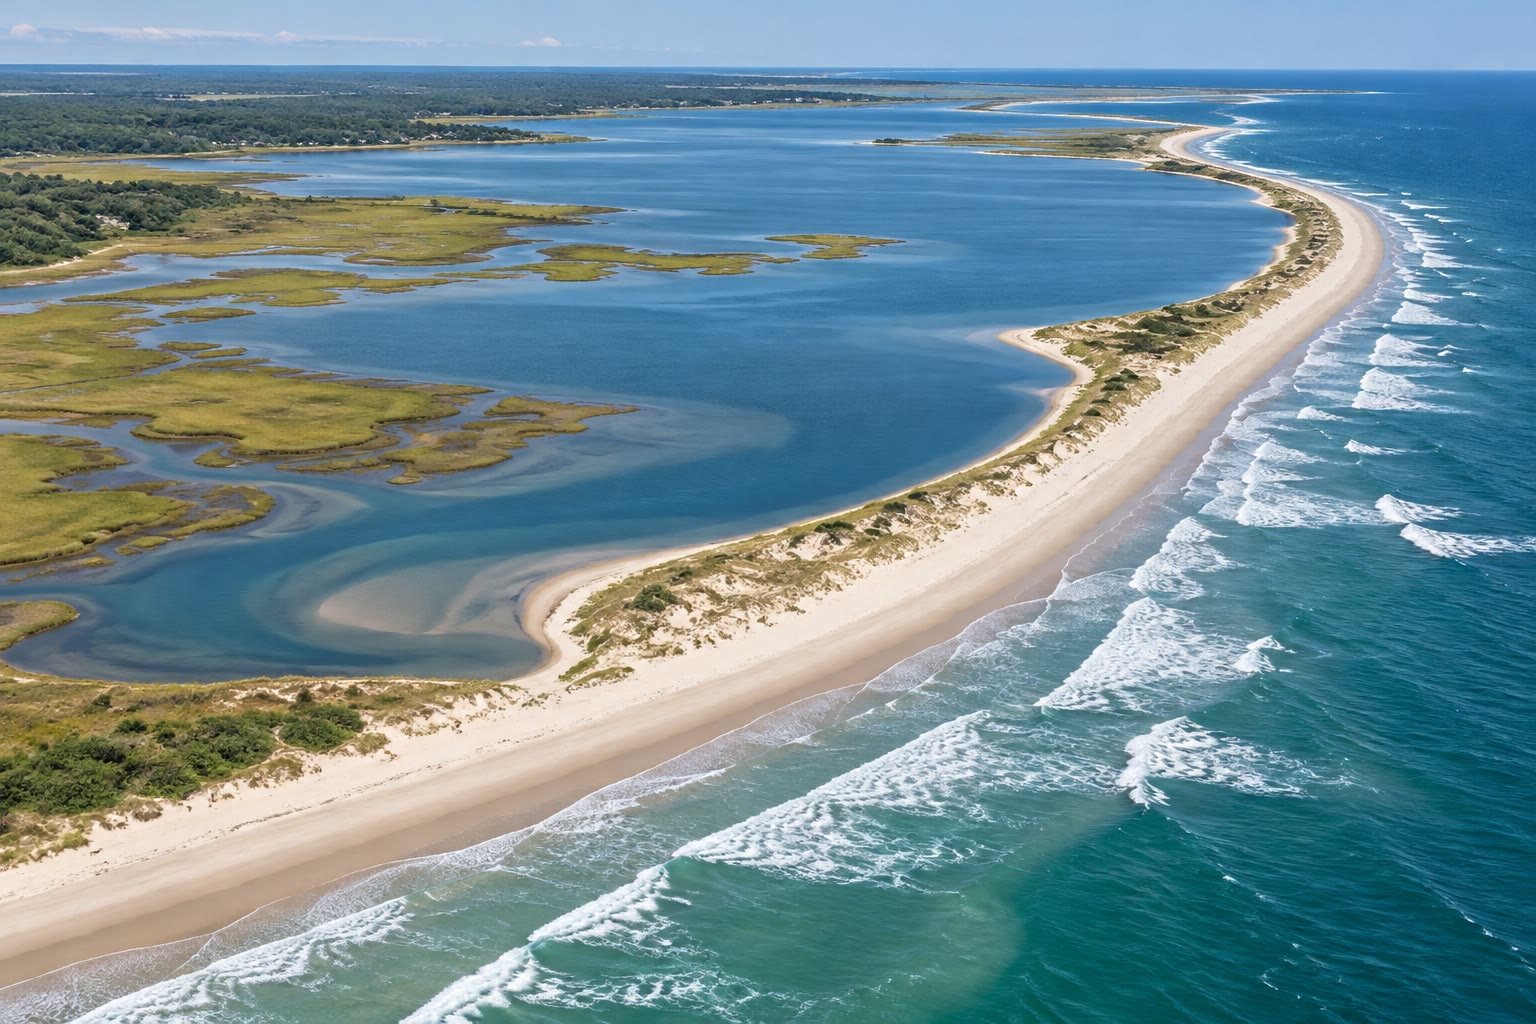
\includegraphics[width=\linewidth]{images/book1/ai/g9-spit-aerial.jpg}
\end{minipage}\hfill
\begin{minipage}[c]{0.46\linewidth}\raggedright
{\small Une flèche de \omterm{def:g3:stones-pebbles-sand:sand}{sable} en travers de l'entrée d'une baie, vue d'un
avion volant bas (une illustration, pas un lieu réel). Les vagues se
brisent sur sa \omterm{def:g9:landforms:beach}{plage} côté \omterm{def:g2:water-on-earth:ocean}{mer}~; derrière elle s'étendent une eau calme et
des prés salés.}
\end{minipage}
\label{fig:g9:landforms:spit-ai}
\end{omfigure}

\section{Les formes de relief dues à la dissolution~: le karst}

L'eau de \omterm{def:g4:clouds-rain-snow:precipitation}{pluie} n'est pas de l'eau pure. En traversant l'air, puis en
s'infiltrant dans le sol, elle se charge de dioxyde de carbone, qui la
rend légèrement acide. Cet acide faible fait lentement ce que la goutte
d'acide dilué fait vite à un morceau de calcaire~: il dissout la \omterm{def:g3:stones-pebbles-sand:rock}{roche}. Le
calcaire est plein de fissures, le long de ses couches et en travers.
L'eau s'y infiltre et les élargit, millimètre par millimètre, pendant des
milliers d'années.
% ledger: usgs:sinkholes, nps:karst

\begin{definition}[Karst, grotte et doline]\label{def:g9:landforms:karst}
Un \emph{karst}\index{karst} est un \omterm{def:g1:landscapes-around-us:landscape}{paysage} façonné par l'eau qui dissout
une \omterm{def:g3:stones-pebbles-sand:rock}{roche} soluble, le plus souvent le calcaire. Les \omterm{def:g1:landscapes-around-us:water}{rivières} y ont
tendance à disparaître sous terre et à ressortir sous forme de \omterm{def:g6:water-underground:spring}{sources}.
Une \emph{grotte}\index{grotte} est un espace souterrain naturel assez
grand pour qu'une personne y entre, creusé par dissolution le long des
fissures de la \omterm{def:g3:stones-pebbles-sand:rock}{roche}. Une \emph{doline}\index{doline} est un creux ou un
trou à la surface du sol, formé là où la \omterm{def:g3:stones-pebbles-sand:rock}{roche} sous-jacente se dissout ou
là où la voûte d'une grotte s'effondre.
\end{definition}
% ledger: nps:karst, usgs:sinkholes

\begin{omfigure}
\begin{tikzpicture}[x=0.9cm, y=0.9cm, font=\footnotesize, >={Stealth[length=2mm]}]
  \pic (B) at (0,0) {blockdiagram={10}{4}{4}};
  % top face: grassland
  \fill[green!25!black!18] (B-ftl) -- (B-ftr) -- (B-btr) -- (B-btl) -- cycle;
  % right face
  \fill[omLithLime!70] (B-fbr) -- (B-bbr) -- (B-btr) -- (B-ftr) -- cycle;
  % front face: limestone layers
  \fill[omLithLime] (B-fbl) rectangle (B-ftr);
  \foreach \y in {0.8,1.6,2.4,3.2} \draw[black!35] (0,\y) -- (10,\y);
  \foreach \x/\y in {1.2/0.8, 3.1/1.6, 4.6/0, 6.8/2.4, 8.3/0.8, 2.2/2.4, 9.1/2.4, 5.6/3.2}
    \draw[black!35] (\x,\y) -- ++(0,0.8);
  % soil
  \fill[brown!45] (0,3.8) rectangle (10,4);
  % sinkhole on the top face and in the front face
  \fill[green!25!black!35] (3.0,4.45) ellipse (0.7 and 0.22);
  \fill[white] (2.3,4) -- (3.7,4) -- (3.25,3.45) -- (2.75,3.45) -- cycle;
  \fill[green!25!black!30] (2.3,4) -- (3.7,4) -- (3.25,3.45) -- (2.75,3.45) -- cycle;
  \draw[black!60] (2.3,4) -- (2.75,3.45) -- (3.25,3.45) -- (3.7,4);
  % shaft from sinkhole to cave
  \fill[white] (2.85,3.45) -- (3.15,3.45) -- (3.35,2.0) -- (3.05,2.0) -- cycle;
  \draw[black!60] (2.85,3.45) -- (3.05,2.0) (3.15,3.45) -- (3.35,2.0);
  % cave
  \fill[white] (2.6,2.1) .. controls (3.5,2.35) and (5.5,2.3) .. (6.6,1.9)
     .. controls (7.4,1.6) and (7.6,1.2) .. (7.2,1.0)
     .. controls (6.0,0.85) and (4.0,1.0) .. (3.0,1.2)
     .. controls (2.3,1.35) and (2.1,1.9) .. (2.6,2.1) -- cycle;
  \draw[black!70] (2.6,2.1) .. controls (3.5,2.35) and (5.5,2.3) .. (6.6,1.9)
     .. controls (7.4,1.6) and (7.6,1.2) .. (7.2,1.0)
     .. controls (6.0,0.85) and (4.0,1.0) .. (3.0,1.2)
     .. controls (2.3,1.35) and (2.1,1.9) .. (2.6,2.1);
  % underground stream at the cave floor
  \fill[omRiver!60] (3.0,1.2) .. controls (4.0,1.0) and (6.0,0.85) .. (7.2,1.0) -- (7.1,1.12)
     .. controls (6.0,1.0) and (4.0,1.12) .. (3.1,1.3) -- cycle;
  % stalactites and stalagmites
  \foreach \x/\l in {4.2/0.35, 4.5/0.22, 4.9/0.4, 5.3/0.25, 5.8/0.3}
    \fill[black!45] (\x-0.07,2.22) -- (\x+0.06,2.22) -- (\x,2.22-\l) -- cycle;
  \foreach \x/\l in {4.9/0.3, 5.8/0.25}
    \fill[black!45] (\x-0.12,0.95) -- (\x+0.12,0.95) -- (\x,0.95+\l) -- cycle;
  % disappearing stream on the top face
  \draw[omRiver, line width=1.2pt] (7.4,4.85) .. controls (6.9,4.5) and (6.4,4.4) .. (6.0,4.25);
  \fill[black!70] (6.0,4.25) circle (0.07);
  \draw[omRiver, dashed, thick] (6.0,4.0) -- (6.4,2.1);
  % spring on the right face
  \draw[omRiver, line width=1.2pt, ->] (10.2,1.2) .. controls (10.8,1.1) and (11.2,0.7) .. (11.6,0.5);
  % rain with carbon dioxide
  \foreach \x in {0.6,1.2,1.8} \draw[->, omRiver] (\x,5.6) -- ++(-0.15,-0.7);
  \draw[->, omRiver, dashed] (1.0,3.9) -- (1.2,1.7);
  % outline
  \draw[black!70] (B-fbl) rectangle (B-ftr);
  \draw[black!70] (B-ftl) -- (B-btl) -- (B-btr) -- (B-ftr) (B-btr) -- (B-bbr) -- (B-fbr);
  % labels
  \node[anchor=south, align=center] at (1.2,5.6) {la pluie se charge en dioxyde\\de carbone~: légèrement acide};
  \node[anchor=east, align=right] at (-0.1,1.6) {l'eau élargit\\les fissures};
  \draw[black!70] (-0.05,1.6) -- (1.1,2.0);
  \node[anchor=south] at (3.0,5.2) {doline};
  \draw[black!70] (3.0,5.2) -- (3.0,4.55);
  \node[anchor=south, align=center] at (7.6,5.3) {un ruisseau disparaît\\sous terre};
  \draw[black!70] (7.0,5.3) -- (6.1,4.35);
  \node[anchor=north, align=center] at (5.0,-0.1) {une grotte~: les stalactites pendent de la voûte,\\les stalagmites montent du sol};
  \draw[black!70] (5.0,-0.1) -- (5.0,1.4);
  \node[anchor=west, align=left] at (11.6,0.6) {source};
  \node[anchor=west] at (11.9,3.4) {calcaire};
\end{tikzpicture}

{\small Un \omterm{def:g1:landscapes-around-us:landscape}{paysage} karstique (un croquis, sans souci d'échelle). Une eau
légèrement acide s'infiltre dans les fissures du calcaire et les élargit~;
des cours d'eau souterrains creusent des \omterm{def:g9:landforms:karst}{grottes}~; la voûte d'une \omterm{def:g9:landforms:karst}{grotte}
cède et ouvre une \omterm{def:g9:landforms:karst}{doline}~; un ruisseau disparaît dans un trou et ressort
plus bas sous forme de \omterm{def:g6:water-underground:spring}{source}.}
% ledger: nps:karst, usgs:sinkholes, nps:speleothems
\label{fig:g9:landforms:karst}
\end{omfigure}

Dans une \omterm{def:g9:landforms:karst}{grotte}, la dissolution peut s'inverser. Une goutte d'eau qui
suinte de la voûte transporte du calcaire dissous. Au contact de l'air de
la \omterm{def:g9:landforms:karst}{grotte}, elle libère une partie de son dioxyde de carbone, et une fine
pellicule de calcite se dépose autour de la goutte. Goutte après goutte, un
tube creux grandit depuis la voûte, puis s'épaissit en une
\emph{stalactite}\index{stalactite}, suspendue comme un glaçon. Là où les
gouttes tombent, le reste de la calcite construit une
\emph{stalagmite}\index{stalagmite} qui monte du sol. Quand les deux se
rejoignent, elles forment une colonne.
% ledger: nps:speleothems

\begin{omfigure}
\begin{minipage}[c]{0.5\linewidth}\centering
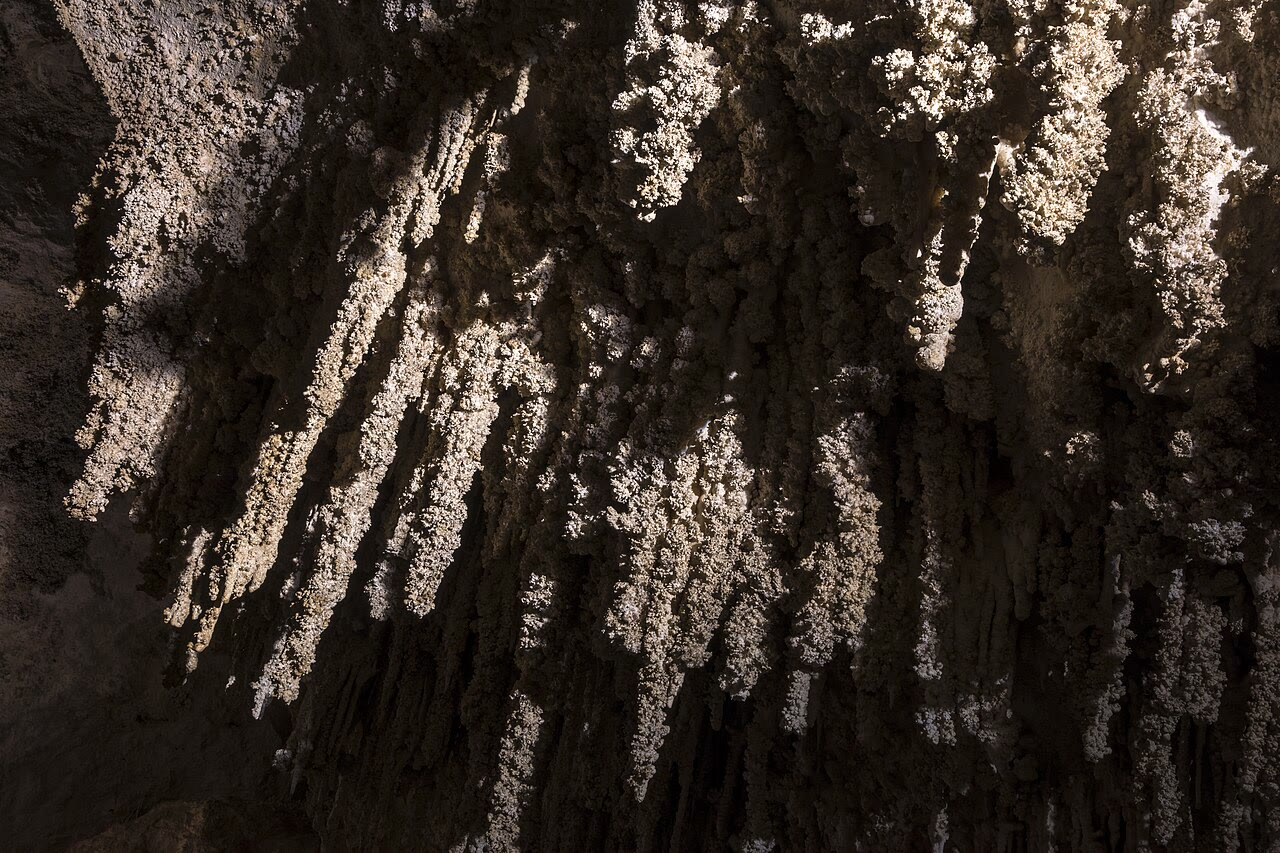
\includegraphics[width=\linewidth]{images/book1/g9-stalactites.jpg}
\end{minipage}\hfill
\begin{minipage}[c]{0.46\linewidth}\raggedright
{\small Des stalactites suspendues sous un gros bloc de \omterm{def:g3:stones-pebbles-sand:rock}{roche} à Carlsbad
Cavern, au Nouveau-Mexique, une \omterm{def:g9:landforms:karst}{grotte} creusée par dissolution dans le
calcaire. Chacune a grandi goutte à goutte à partir de l'eau qui
s'infiltre dans la \omterm{def:g3:stones-pebbles-sand:rock}{roche} au-dessus. National Park Service, 2018 (domaine
public, via Wikimedia Commons).}
\end{minipage}
% ledger: commons:carlsbad-stalactites, nps:speleothems
\label{fig:g9:landforms:stalactites}
\end{omfigure}

Une région karstique contient beaucoup d'\omterm{def:g6:water-underground:groundwater}{eau souterraine}, mais celle-ci
circule vite dans les fissures ouvertes et n'est presque pas filtrée~: ce
qui est déversé sur le sol peut atteindre rapidement une \omterm{def:g6:water-underground:spring}{source}. Et là où
la \omterm{def:g3:stones-pebbles-sand:rock}{roche} sous-jacente a été dissoute, le sol peut s'affaisser ou
s'effondrer~: là où des gens habitent, une \omterm{def:g9:landforms:karst}{doline} qui s'ouvre soudain peut
engloutir des routes et des maisons.
% ledger: nps:karst, usgs:sinkholes

\section{Lire un paysage}

Chaque \omterm{def:g1:landscapes-around-us:landform}{forme de relief} est un indice. Sa forme dit quel agent l'a
façonnée~; l'agent dit quel processus était à l'œuvre, \omterm{def:g5:water-shapes-the-land:erosion}{érosion} ou \omterm{def:g5:water-shapes-the-land:deposition}{dépôt}~;
et le processus renseigne souvent sur la \omterm{def:g3:stones-pebbles-sand:rock}{roche} ou les matériaux meubles
situés dessous.

\begin{method}[Lire une forme de relief]
\begin{enumerate}
  \item \textbf{Forme.} Décris la \omterm{def:g1:landscapes-around-us:landform}{forme de relief}~: une crête, un creux,
        une paroi raide, un replat~; sa taille~; dans quelle direction elle
        pointe.
  \item \textbf{Agent et processus.} Détermine quel agent l'a façonnée (une
        \omterm{def:g1:landscapes-around-us:water}{rivière}, la glace, le vent, la \omterm{def:g2:water-on-earth:ocean}{mer}, l'eau qui dissout) et si elle a
        été creusée (\omterm{def:g5:water-shapes-the-land:erosion}{érosion}) ou construite (\omterm{def:g5:water-shapes-the-land:deposition}{dépôt}).
  \item \textbf{Matériau.} Dis de quoi elle est faite, ou quelle est
        probablement la \omterm{def:g3:stones-pebbles-sand:rock}{roche} dessous~: \omterm{def:g3:stones-pebbles-sand:sand}{sable} meuble, \omterm{def:g3:stones-pebbles-sand:pebble}{galets}, calcaire,
        \omterm{def:g3:stones-pebbles-sand:rock}{roche} dure ou tendre.
\end{enumerate}
\end{method}

\begin{center}
{\small
\begin{tabular}{|>{\raggedright\arraybackslash}p{4.6cm}|>{\raggedright\arraybackslash}p{2.6cm}|>{\raggedright\arraybackslash}p{2.2cm}|>{\raggedright\arraybackslash}p{2.6cm}|}
\hline
forme & agent & processus & matériau \\
\hline
\omterm{def:g1:landscapes-around-us:landform}{collines} de \omterm{def:g3:stones-pebbles-sand:sand}{sable} en forme de croissant & vent & \omterm{def:g5:water-shapes-the-land:deposition}{dépôt} & \omterm{def:g3:stones-pebbles-sand:sand}{sable} meuble \\
une paroi rocheuse verticale au-dessus d'un replat rocheux & \omterm{def:g2:water-on-earth:ocean}{mer} & \omterm{def:g5:water-shapes-the-land:erosion}{érosion} & \omterm{def:g3:stones-pebbles-sand:rock}{roche} (la \omterm{def:g3:stones-pebbles-sand:rock}{roche} tendre recule vite) \\
une étroite crête de \omterm{def:g3:stones-pebbles-sand:sand}{sable} en travers d'une baie & \omterm{def:g2:water-on-earth:ocean}{mer} (\omterm{def:g9:landforms:beach}{dérive littorale}) & \omterm{def:g5:water-shapes-the-land:deposition}{dépôt} & \omterm{def:g3:stones-pebbles-sand:sand}{sable} ou \omterm{def:g3:stones-pebbles-sand:pebble}{galets} \\
des creux dans les champs, des ruisseaux qui disparaissent & eau qui dissout & dissolution & calcaire \\
une \omterm{def:g8:ice-on-earth:glacial-landforms}{vallée en U} & glace & \omterm{def:g5:water-shapes-the-land:erosion}{érosion} & toute \omterm{def:g3:stones-pebbles-sand:rock}{roche} \\
un éventail de \omterm{def:g3:stones-pebbles-sand:sand}{boue} à l'\omterm{def:g5:water-shapes-the-land:source-mouth}{embouchure} d'une \omterm{def:g1:landscapes-around-us:water}{rivière} & \omterm{def:g1:landscapes-around-us:water}{rivière} & \omterm{def:g5:water-shapes-the-land:deposition}{dépôt} & \omterm{def:g3:stones-pebbles-sand:sand}{boue} et \omterm{def:g3:stones-pebbles-sand:sand}{sable} \\
\hline
\end{tabular}}
\end{center}

\begin{example}[Une promenade sur un plateau]
Sur un haut plateau herbeux, il n'y a aucun ruisseau, bien qu'il pleuve
souvent. Les champs sont parsemés de creux arrondis de quelques mètres de
diamètre, et, dans la \omterm{def:g1:landscapes-around-us:landform}{vallée} en contrebas, une puissante \omterm{def:g6:water-underground:spring}{source} jaillit au
pied d'une paroi rocheuse. \emph{Forme}~: des creux, aucun cours d'eau en
surface, une \omterm{def:g6:water-underground:spring}{source} plus bas. \emph{Agent et processus}~: de l'eau qui
dissout la \omterm{def:g3:stones-pebbles-sand:rock}{roche} et circule sous terre. \emph{Matériau}~: le plateau est
très probablement calcaire, et les creux sont des \omterm{def:g9:landforms:karst}{dolines}. Une goutte
d'acide dilué déposée par le professeur sur un morceau de \omterm{def:g3:stones-pebbles-sand:rock}{roche} détaché
ferait effervescence.
\end{example}
% ledger: nps:karst, usgs:sinkholes

\section{Exercices}

\begin{exercise}[$\star$]\label{exo:g9:landforms:1}
Quel agent a façonné chaque \omterm{def:g1:landscapes-around-us:landform}{forme de relief}~: le vent, la \omterm{def:g2:water-on-earth:ocean}{mer}, une
\omterm{def:g1:landscapes-around-us:water}{rivière}, la glace, ou l'eau qui dissout la \omterm{def:g3:stones-pebbles-sand:rock}{roche}~? (a) Une \omterm{def:g1:landscapes-around-us:landform}{colline} de
\omterm{def:g3:stones-pebbles-sand:sand}{sable} en forme de croissant dans un \omterm{def:g5:weather-and-climate:desert}{désert}. (b) Une \omterm{def:g9:landforms:karst}{grotte} pleine de
stalactites. (c) Une longue crête de \omterm{def:g3:stones-pebbles-sand:pebble}{galets} en travers de l'entrée d'une
baie. (d) Une \omterm{def:g8:ice-on-earth:glacial-landforms}{vallée en U} avec une \omterm{def:g8:ice-on-earth:glacial-landforms}{moraine} à son extrémité. (e) Une paroi
de craie verticale avec un replat rocheux à son pied. (f) Un \omterm{def:g5:water-shapes-the-land:delta}{delta}.
\end{exercise}

\begin{exercise}[$\star$]\label{exo:g9:landforms:2}
Donne le mot qui correspond à chaque description. (a) La lente élévation
des \omterm{def:g3:stones-pebbles-sand:rock}{roches} et du sol d'une région. (b) Le versant raide d'une \omterm{def:g9:landforms:dune}{dune}, à
l'abri du vent. (c) Un trou dans le sol formé là où la \omterm{def:g3:stones-pebbles-sand:rock}{roche} sous-jacente
s'est dissoute ou là où la voûte d'une \omterm{def:g9:landforms:karst}{grotte} s'est effondrée. (d) Le
déplacement du \omterm{def:g3:stones-pebbles-sand:sand}{sable} et des \omterm{def:g3:stones-pebbles-sand:pebble}{galets} le long du rivage. (e) Un \omterm{def:g1:landscapes-around-us:landscape}{paysage}
façonné par l'eau qui dissout le calcaire.
\end{exercise}

\begin{exercise}[$\star$]\label{exo:g9:landforms:3}
Vrai ou faux~? Corrige les phrases fausses. (a) Les cornes d'une \omterm{def:g9:landforms:dune}{dune} en
croissant pointent vers le vent. (b) La pente d'une \omterm{def:g9:landforms:dune}{dune} tournée vers le
vent est douce. (c) Une \omterm{def:g9:landforms:dune}{dune} avance parce que le vent la soulève tout
entière d'un coup. (d) Les \omterm{def:g9:landforms:dune}{dunes} se forment plus facilement là où peu de
plantes poussent.
\end{exercise}

\begin{exercise}[$\star$]\label{exo:g9:landforms:4}
Remets dans l'ordre ces étapes du recul d'une \omterm{def:g9:landforms:cliff}{falaise} littorale. (a) Les
vagues brisent les blocs tombés et les emportent. (b) Les vagues creusent
une encoche au pied de la \omterm{def:g9:landforms:cliff}{falaise}. (c) La paroi de la \omterm{def:g9:landforms:cliff}{falaise} se trouve
maintenant plus loin vers l'intérieur, et la plate-forme rocheuse devant
elle est un peu plus large. (d) La \omterm{def:g3:stones-pebbles-sand:rock}{roche} au-dessus de l'encoche forme un
surplomb. (e) Le surplomb s'effondre.
\end{exercise}

\begin{exercise}[$\star\star$]\label{exo:g9:landforms:5}
% ledger: nps:whsa-migration (6 and 3 m a year)
Vues d'avion, les \omterm{def:g9:landforms:dune}{dunes} en croissant d'un \omterm{def:g5:weather-and-climate:desert}{désert} ont toutes leurs cornes
tournées vers l'est. (a) De quelle direction souffle le vent~? (b) De
quel côté de chaque \omterm{def:g9:landforms:dune}{dune} se trouve la \omterm{def:g9:landforms:dune}{face d'avalanche}~? (c) Une route
passe à \qty{60}{m} à l'est de l'une des \omterm{def:g9:landforms:dune}{dunes}. La \omterm{def:g9:landforms:dune}{dune} avance de
\qty{6}{m} par an. Dans combien d'années son pied atteindra-t-il la
route~? (d) Une \omterm{def:g9:landforms:dune}{dune} plus grande n'avance que de \qty{3}{m} par an.
Pourquoi les grandes \omterm{def:g9:landforms:dune}{dunes} avancent-elles plus lentement~?
\end{exercise}

\begin{exercise}[$\star\star$]\label{exo:g9:landforms:6}
% ledger: sdnp:birling, nt:birling-2014
Les \omterm{def:g9:landforms:cliff}{falaises} de craie d'une \omterm{def:g1:landscapes-around-us:water}{côte} reculent de jusqu'à environ \qty{1}{m}
par an. Pendant l'hiver 2014, elles ont perdu autant qu'elles perdent
d'habitude en sept ans, en deux mois seulement. (a) À \qty{1}{m} par an,
combien perdent-elles en sept ans~? (b) Deux mois représentent quelle
fraction d'une année~? (c) Combien de fois plus vite que d'habitude les
\omterm{def:g9:landforms:cliff}{falaises} ont-elles reculé pendant ces deux mois~? (d) Explique, à l'aide
de l'encoche et du surplomb, pourquoi une \omterm{def:g9:landforms:cliff}{falaise} recule par à-coups
plutôt que régulièrement.
\end{exercise}

\begin{exercise}[$\star\star$]\label{exo:g9:landforms:7}
Une \omterm{def:g1:landscapes-around-us:water}{côte} rectiligne s'étend d'ouest en est, avec la \omterm{def:g2:water-on-earth:ocean}{mer} au sud. Les vagues
viennent du sud-ouest. (a) Dans quelle direction la \omterm{def:g9:landforms:beach}{dérive littorale}
emporte-t-elle le \omterm{def:g3:stones-pebbles-sand:sand}{sable}~? (b) Dessine le trajet en zigzag d'un \omterm{def:g3:stones-pebbles-sand:pebble}{galet} sur
trois vagues, en légendant la montée sur la \omterm{def:g9:landforms:beach}{plage} et le retour vers le
bas. (c) À son extrémité est, la \omterm{def:g1:landscapes-around-us:water}{côte} tourne vers le nord pour former une
baie. Quelle \omterm{def:g1:landscapes-around-us:landform}{forme de relief} risque de s'y développer~? (d) Pourquoi la
vase se dépose-t-elle derrière elle~?
\end{exercise}

\begin{exercise}[$\star\star$]\label{exo:g9:landforms:8}
(a) Qu'est-ce qui rend l'eau de \omterm{def:g4:clouds-rain-snow:precipitation}{pluie} légèrement acide~? (b) Pourquoi
trouve-t-on des \omterm{def:g9:landforms:karst}{grottes} dans le calcaire mais presque aucune dans le
granite~? (c) Pourquoi les \omterm{def:g9:landforms:karst}{grottes} suivent-elles les fissures et les
couches de la \omterm{def:g3:stones-pebbles-sand:rock}{roche}~? (d) Donne deux façons dont une \omterm{def:g9:landforms:karst}{doline} peut se
former.
\end{exercise}

\begin{exercise}[$\star\star$]\label{exo:g9:landforms:9}
(a) Explique pourquoi de la calcite se dépose à partir d'une goutte d'eau
suspendue à la voûte d'une \omterm{def:g9:landforms:karst}{grotte}. (b) Pourquoi les stalagmites n'ont-elles
pas de tube creux à l'intérieur, contrairement aux jeunes stalactites~?
(c) Suppose qu'une stalactite ait grandi de \qty{0.1}{mm} par an (un
rythme inventé~: les rythmes réels varient beaucoup). Combien d'années
lui a-t-il fallu pour atteindre \qty{30}{cm}~? Écris la réponse en
notation scientifique.
\end{exercise}

\begin{exercise}[$\star\star$]\label{exo:g9:landforms:10}
% ledger: usgs:himalaya, sdnp:birling
Le plateau du Tibet s'est élevé d'environ \qty{4600}{m} en environ
10~millions d'années. (a) Calcule le \omterm{def:g9:landforms:uplift}{soulèvement} moyen en mètres par an,
en notation scientifique, puis en millimètres par an. (b) Suppose que
l'\omterm{def:g5:water-shapes-the-land:erosion}{érosion} enlève \qty{0.2}{mm} par an au plateau (un chiffre inventé). De
combien le plateau s'élève-t-il chaque année~? (c) Une \omterm{def:g9:landforms:cliff}{falaise} de craie
recule d'environ \qty{1}{m} par an. Combien de fois plus vite que le
\omterm{def:g9:landforms:uplift}{soulèvement} de (a) cela fait-il~? (d) Pourquoi un \omterm{def:g9:landforms:uplift}{soulèvement} lent
peut-il tout de même construire un haut plateau~?
\end{exercise}

\begin{exercise}[$\star\star\star$]\label{exo:g9:landforms:11}
Lis chaque \omterm{def:g1:landscapes-around-us:landscape}{paysage} avec la méthode du chapitre (forme, agent et processus,
matériau). (a) Dans un pays sec, de longues files de \omterm{def:g1:landscapes-around-us:landform}{collines} de \omterm{def:g3:stones-pebbles-sand:sand}{sable},
chacune en forme de croissant, avec un versant raide tourné vers le
sud-est. (b) Au pied d'une \omterm{def:g9:landforms:cliff}{falaise} blanche, un replat rocheux couvert
d'algues apparaît à marée basse. (c) Sur un vaste plateau de \omterm{def:g3:stones-pebbles-sand:rock}{roche}
claire, un ruisseau traverse un champ et disparaît dans un trou~; une
\omterm{def:g6:water-underground:spring}{source} jaillit d'un versant de \omterm{def:g1:landscapes-around-us:landform}{vallée} à \qty{2}{km} de là.
\end{exercise}

\begin{exercise}[$\star\star\star$]\label{exo:g9:landforms:12}
% ledger: nps:whsa-migration, nmt:barchan, nps:aeolian
Dans un champ de \omterm{def:g9:landforms:dune}{dunes}, les petites \omterm{def:g9:landforms:dune}{dunes} du bord exposé au vent avancent
jusqu'à \qty{6}{m} par an~; un peu plus loin, les \omterm{def:g9:landforms:dune}{dunes}, hautes de 6 à
\qty{10}{m}, avancent d'environ \qty{3}{m} par an. Une piste traverse le
champ à \qty{45}{m} sous le vent d'une \omterm{def:g9:landforms:dune}{dune} de chaque sorte. (a) Au bout
de combien d'années chaque \omterm{def:g9:landforms:dune}{dune} atteint-elle la piste~? (b) Des \omterm{def:g9:landforms:dune}{dunes}
poussées par des vents forts peuvent parcourir plus de \qty{100}{m} en un
an. Combien de temps une telle \omterm{def:g9:landforms:dune}{dune} mettrait-elle pour parcourir la même
distance~? (c) Nomme un moyen de ralentir les \omterm{def:g9:landforms:dune}{dunes}, et explique comment
il agit.
\end{exercise}

\section{Problème~: la falaise et la route côtière}

\begin{problem}[{Problème du week-end --- une route côtière longe une
falaise de craie qui recule~; la réponse finale est l'année où le bord de
la falaise atteindrait la route au rythme mesuré}]
\label{pb:g9:landforms:1}
% ledger: (invented region: exercise data, figdata/grade-9/cliff_retreat.py; the rate is kept within sdnp:birling, the storm winter recalls nt:birling-2014)
Une route côtière longe le haut de \omterm{def:g9:landforms:cliff}{falaises} de craie. Régulièrement, une
équipe de géomètres mesure la distance de la route au bord de la \omterm{def:g9:landforms:cliff}{falaise}
le long d'une même ligne, à partir de repères fixes placés bien en
retrait du bord, jamais au bord lui-même. Voici ses mesures.

\begin{center}
{\small
\begin{tabular}{|l|c|c|c|c|c|c|c|}
\hline
année & 2004 & 2008 & 2012 & 2014 & 2016 & 2020 & 2024 \\
\hline
distance de la route au bord (m) & 46.0 & 43.1 & 41.0 & 36.2 & 35.5 & 33.0 & 30.4 \\
\hline
\end{tabular}}
\end{center}

\noindent\textbf{Partie I --- Les mesures.}\par\nopagebreak
\begin{enumerate}[beginpenalty=10000]
  \item De combien de mètres le bord de la \omterm{def:g9:landforms:cliff}{falaise} s'est-il rapproché de
        la route entre 2004 et 2024~?
  \item Calcule le rythme moyen de recul sur ces 20 ans, en mètres par an.
  \item Entre quelles deux mesures le bord a-t-il reculé le plus vite~?
        Calcule le rythme sur cet intervalle.
  \item Combien de fois plus rapide que la moyenne est-il~? Propose une
        explication de ce qui s'est passé pendant cet intervalle.
\end{enumerate}

\begin{omfigure}
\begin{tikzpicture}
\begin{axis}[omrecord, width=11cm, height=4.6cm, xmin=2000, xmax=2070,
  ymin=0, ymax=50, xtick={2000,2010,...,2070}, ytick={0,10,...,50},
  x tick label style={/pgf/number format/1000 sep={}},
  xlabel={année}, ylabel={distance à la route (m)}]
  \addplot[omWarm, thick, mark=*, mark size=1.8pt] table[x=year, y=dist_m] {figdata/out/grade-9-cliff_retreat.dat};
\end{axis}
\end{tikzpicture}

{\small Les mesures~: distance de la route côtière au bord de la \omterm{def:g9:landforms:cliff}{falaise}
(données d'exercice).}
\label{fig:g9:landforms:survey}
\end{omfigure}

\noindent\textbf{Partie II --- Le rythme.}\par\nopagebreak
\begin{enumerate}[resume, beginpenalty=10000]
  \item Écris le rythme moyen en centimètres par an, puis en mètres par
        siècle.
  \item Sur une vraie \omterm{def:g1:landscapes-around-us:water}{côte} de craie, les \omterm{def:g9:landforms:cliff}{falaises} reculent jusqu'à environ
        un mètre par an. Le recul de cette \omterm{def:g9:landforms:cliff}{falaise} est-il du même ordre~?
  \item Un phare d'une telle \omterm{def:g1:landscapes-around-us:water}{côte} a autrefois été déplacé de \qty{17}{m}
        vers l'arrière. Au rythme moyen de cette \omterm{def:g9:landforms:cliff}{falaise}, combien d'années
        de recul \qty{17}{m} représentent-ils~?
  \item Pourquoi le rythme mesuré sur 20 ans est-il un meilleur guide pour
        l'avenir que le rythme mesuré sur deux ans~?
\end{enumerate}

\noindent\textbf{Partie III --- La route.}\par\nopagebreak
\begin{enumerate}[resume, beginpenalty=10000]
  \item La route doit être déplacée avant que le bord n'arrive à moins de
        \qty{10}{m} d'elle. En quelle année, au rythme moyen, cela
        arrivera-t-il~?
  \item Si des hivers plus orageux doublaient le rythme, en quelle année le
        bord atteindrait-il la route~?
  \item Pourquoi l'équipe prend-elle ses mesures à partir de repères placés
        bien en retrait du bord~?
  \item Au rythme moyen, en quelle année le bord de la \omterm{def:g9:landforms:cliff}{falaise}
        atteindrait-il la route~?
\end{enumerate}
\end{problem}
